\chapter{予備実験}
\label{CExperiment}

\section{実験の目的}
\label{SExperimentPurpose}


実際の複眼の構造や形状は複雑であり、コンピュータグラフィックスにおいて実物の形状を作成したり、実物の構造計算に用いることは難しい。
そこで、複眼の性質を表現するために代替となる形状や近似モデルが必要となる。
本研究では、永田\cite{永田敏夫:2008-03-10}が行った偽瞳孔の再現実験をもとにビー玉とパンチングメタルを用いて予備実験を行った。

本実験における第一の目的は、 偽瞳孔の発生原理を理解し、物理現象に落としこむことである。
複眼を扱った関連研究のうち、偽瞳孔の性質や現象について生物学上の考察や解説を行うものは存在するものの、幾何学的なしくみについて言及したものは少ない。
そのため、実物を観察することによって物理現象としてのしくみを明らかにし、開発の足がかりとする必要があった。
第二の目的は、実装を行う前に近似手法による偽瞳孔の再現度を確認することである。
永田の実験は複眼の形状を大きく変え、平板と球体として近似している。そのため、コンピュータグラフィックスとして表現するにあたり、適切な手法であることを確認することが望ましい。
そして第三の目的は、レンズや色素細胞に相当するパンチングメタルの穴などの大きさや周期の違いが模様に与える変化を観察することである。
実際の昆虫などの複眼は各個眼の大きさが決まっており、全体の形状に対して自由に個眼の大きさを変化させることができない。
ゆえに、大きさや周期といったパラメータの変化に対して偽瞳孔の模様が変化する様子を確認するために模型を利用する。

\section{実験方法}
\label{SExperimentMethod}

実験に用いた材料は以下のとおりである\figref{FExpparts}。

\begin{itemize}
\item ビー玉(透明なもの)
\item パンチングメタル(穴の大きさと周期の違うもの2種類)
\item 黒色の画用紙
\item 木の棒
\end{itemize}

%% \begin{figure}[htbp]
%%   \centering
%%   \includegraphics[width=3.5in]{./img/exp_asemble_parts.jpg}
%%   \caption{実験の材料}
%%   \label{FExpparts}
%% \end{figure}

\noindent
まず、画用紙とパンチングメタルをセロハンテープなどで固定する\figref{FExpMetalBlack}。
これは、偽瞳孔の模様をはっきりとさせるためにパンチングメタルの穴の部分を黒く見せるためである。
このモデルでは、パンチングメタルの穴が複眼の色素細胞に相当し、ビー玉が個眼のレンズに相当する。
続いて、ビー玉をパンチングメタルの上に配置し、球体レンズによる光の屈折がどのような像を生み出すのかを確認する。
ビー玉をひとつのみ配置した場合、木枠により複数のビー玉を密集させた場合、そしてビー玉とパンチングメタルの穴の配置を合わせた場合のそれぞれについてビー玉に写る像の観察を行った。
木枠を用いる場合では、まず木の棒で枠を作ってパンチングメタルの上に乗せ、木の枠内にできるだけ隙間が開かないようにビー玉を敷き詰める。
実際の複眼では個眼のそれぞれにおいて色素細胞とレンズは対応しており同じ周期で配置されているが、木枠を用いる場合では厳密にパンチングメタルの穴の位置とビー玉の配置を一致させてはいない。
ビー玉とパンチングメタルの穴の配置を合わせた場合では、パンチングメタルの穴の直上に必ずビー玉が乗るようにし、複数のビー玉が整列するようになっている。

%% \begin{figure}[htbp]
%%   \centering
%%   \includegraphics[width=3.5in]{./img/exp_metal_black.jpg}
%%   \caption{パンチングメタルを画用紙に固定}
%%   \label{FExpMetalBlack}
%% \end{figure}


\section{結果と議論}
\label{SExperimentResult}

使用したパンチングメタルの大きさは、穴同士の距離が約3.0mmで穴の径が約1.0mmのものと穴同士の距離が約3.5mmで穴の径が約1.5mmのもの。
ビー玉は径が約12.0mmおよび約8.0mmのものを使用した。
木の棒はそれぞれ幅15.0mm、高さ15.0mm、奥行き200.0mmのもの4本を加工して木の枠を作成した\figref{FExpparts}。
また、パンチングメタルの大きさとビー玉の大きさがそれぞれ2種類ずつあるため、これらを組み合わせたモデルに対して観察を行った。

\subsection{ビー玉がひとつの場合}
\label{SSOnemarble}
まずはじめに、ひとつのビー玉をパンチングメタルの穴の直上に置いて、ビー玉表面に写る像を観察した。
パンチングメタルを正面に近い方向から見ると、黒点(パンチングメタルの穴)が拡大された虚像を確認することができた\figref{}。
さらに、レンズを見る角度を変えてパンチングメタルと平行に近づけていくと、ある角度を境に倒立像が観測されるようになった\figref{}。
また、球の直下の黒点を像として写した場合よりも、隣接した黒点を写した際に球に占める黒い部分が大きくなるという結果が得られた\figref{}。
すなわち、穴の正面からビー玉を見る場合よりもある程度角度をつけた場合のほうがビー玉全体が黒く見える。
以上から、球の直下およびその周辺の黒点に対してビー玉が拡大レンズとして作用していることが確認できた。

%% \begin{figure}[htbp]
%%   \centering
%% \subfigure[CAPTIONa]{
%% \includegraphics*[width=.45\columnwidth]{./img/exp_first_kakudai.jpg}
%% \label{fig:it-PP}}
%% \subfigure[CAPTIONb]{
%% \includegraphics*[width=.45\columnwidth]{./img/exp_second_kakudai.jpg}
%% \label{fig:st-PP}}\\
%% \subfigure[CAPTIONc]{
%% \includegraphics*[width=.45\columnwidth]{./img/exp_touritsu.jpg}
%% \label{fig:at-PP}}
%%   \caption{}
%%   \label{FExp}
%% \end{figure}

\subsection{木枠を用いてビー玉を密集させた場合}
\label{SSWoodframe}

%% \begin{figure}[htbp]
%%   \centering
%%   \includegraphics[width=3.5in]{./img/exp_wood.jpg}
%%   \caption{}
%%   \label{FExpWood}
%% \end{figure}

続いて、木枠を用いてビー玉を密集して配置した\figref{}。
この場合、ビー玉の直下にパンチングメタルの穴があるとは限らないため、各ビー玉ごとに写る像の違いが大きいことに注意する。
ビー玉の大きさを変えても特に大きな違いはなく、各パンチングメタルを拡大した虚像が観測され、生じる像の周期はパンチングメタルの大きさによって変化した\figref{}。
パンチングメタル上のビー玉を木枠と共に動かすことによって、拡大された黒点が流れるように動く様子を肉眼で確認することができる。
このことから、球体レンズを密集させることによって奥で接している面上の様子を拡大できることを確認した。

\subsection{ビー玉とパンチングメタルの穴の配置を合わせた場合}
\label{SSMarbleOnHole}
前述の木枠を用いた方法ではビー玉の周期とパンチングメタルの穴の周期が一致しておらず、球の直下に必ずパンチングメタルの穴を配置することはできなかった。
そこで、穴同士の距離と級の直径がおおむね一致する、径が約12.0mmのビー玉および穴同士の距離が約3.5mmで穴の径が約1.5mmのパンチングメタルを用いて球の直下に必ず黒点が来るような配置を作成した\figref{}。

%% \begin{figure}[htbp]
%%   \centering
%%   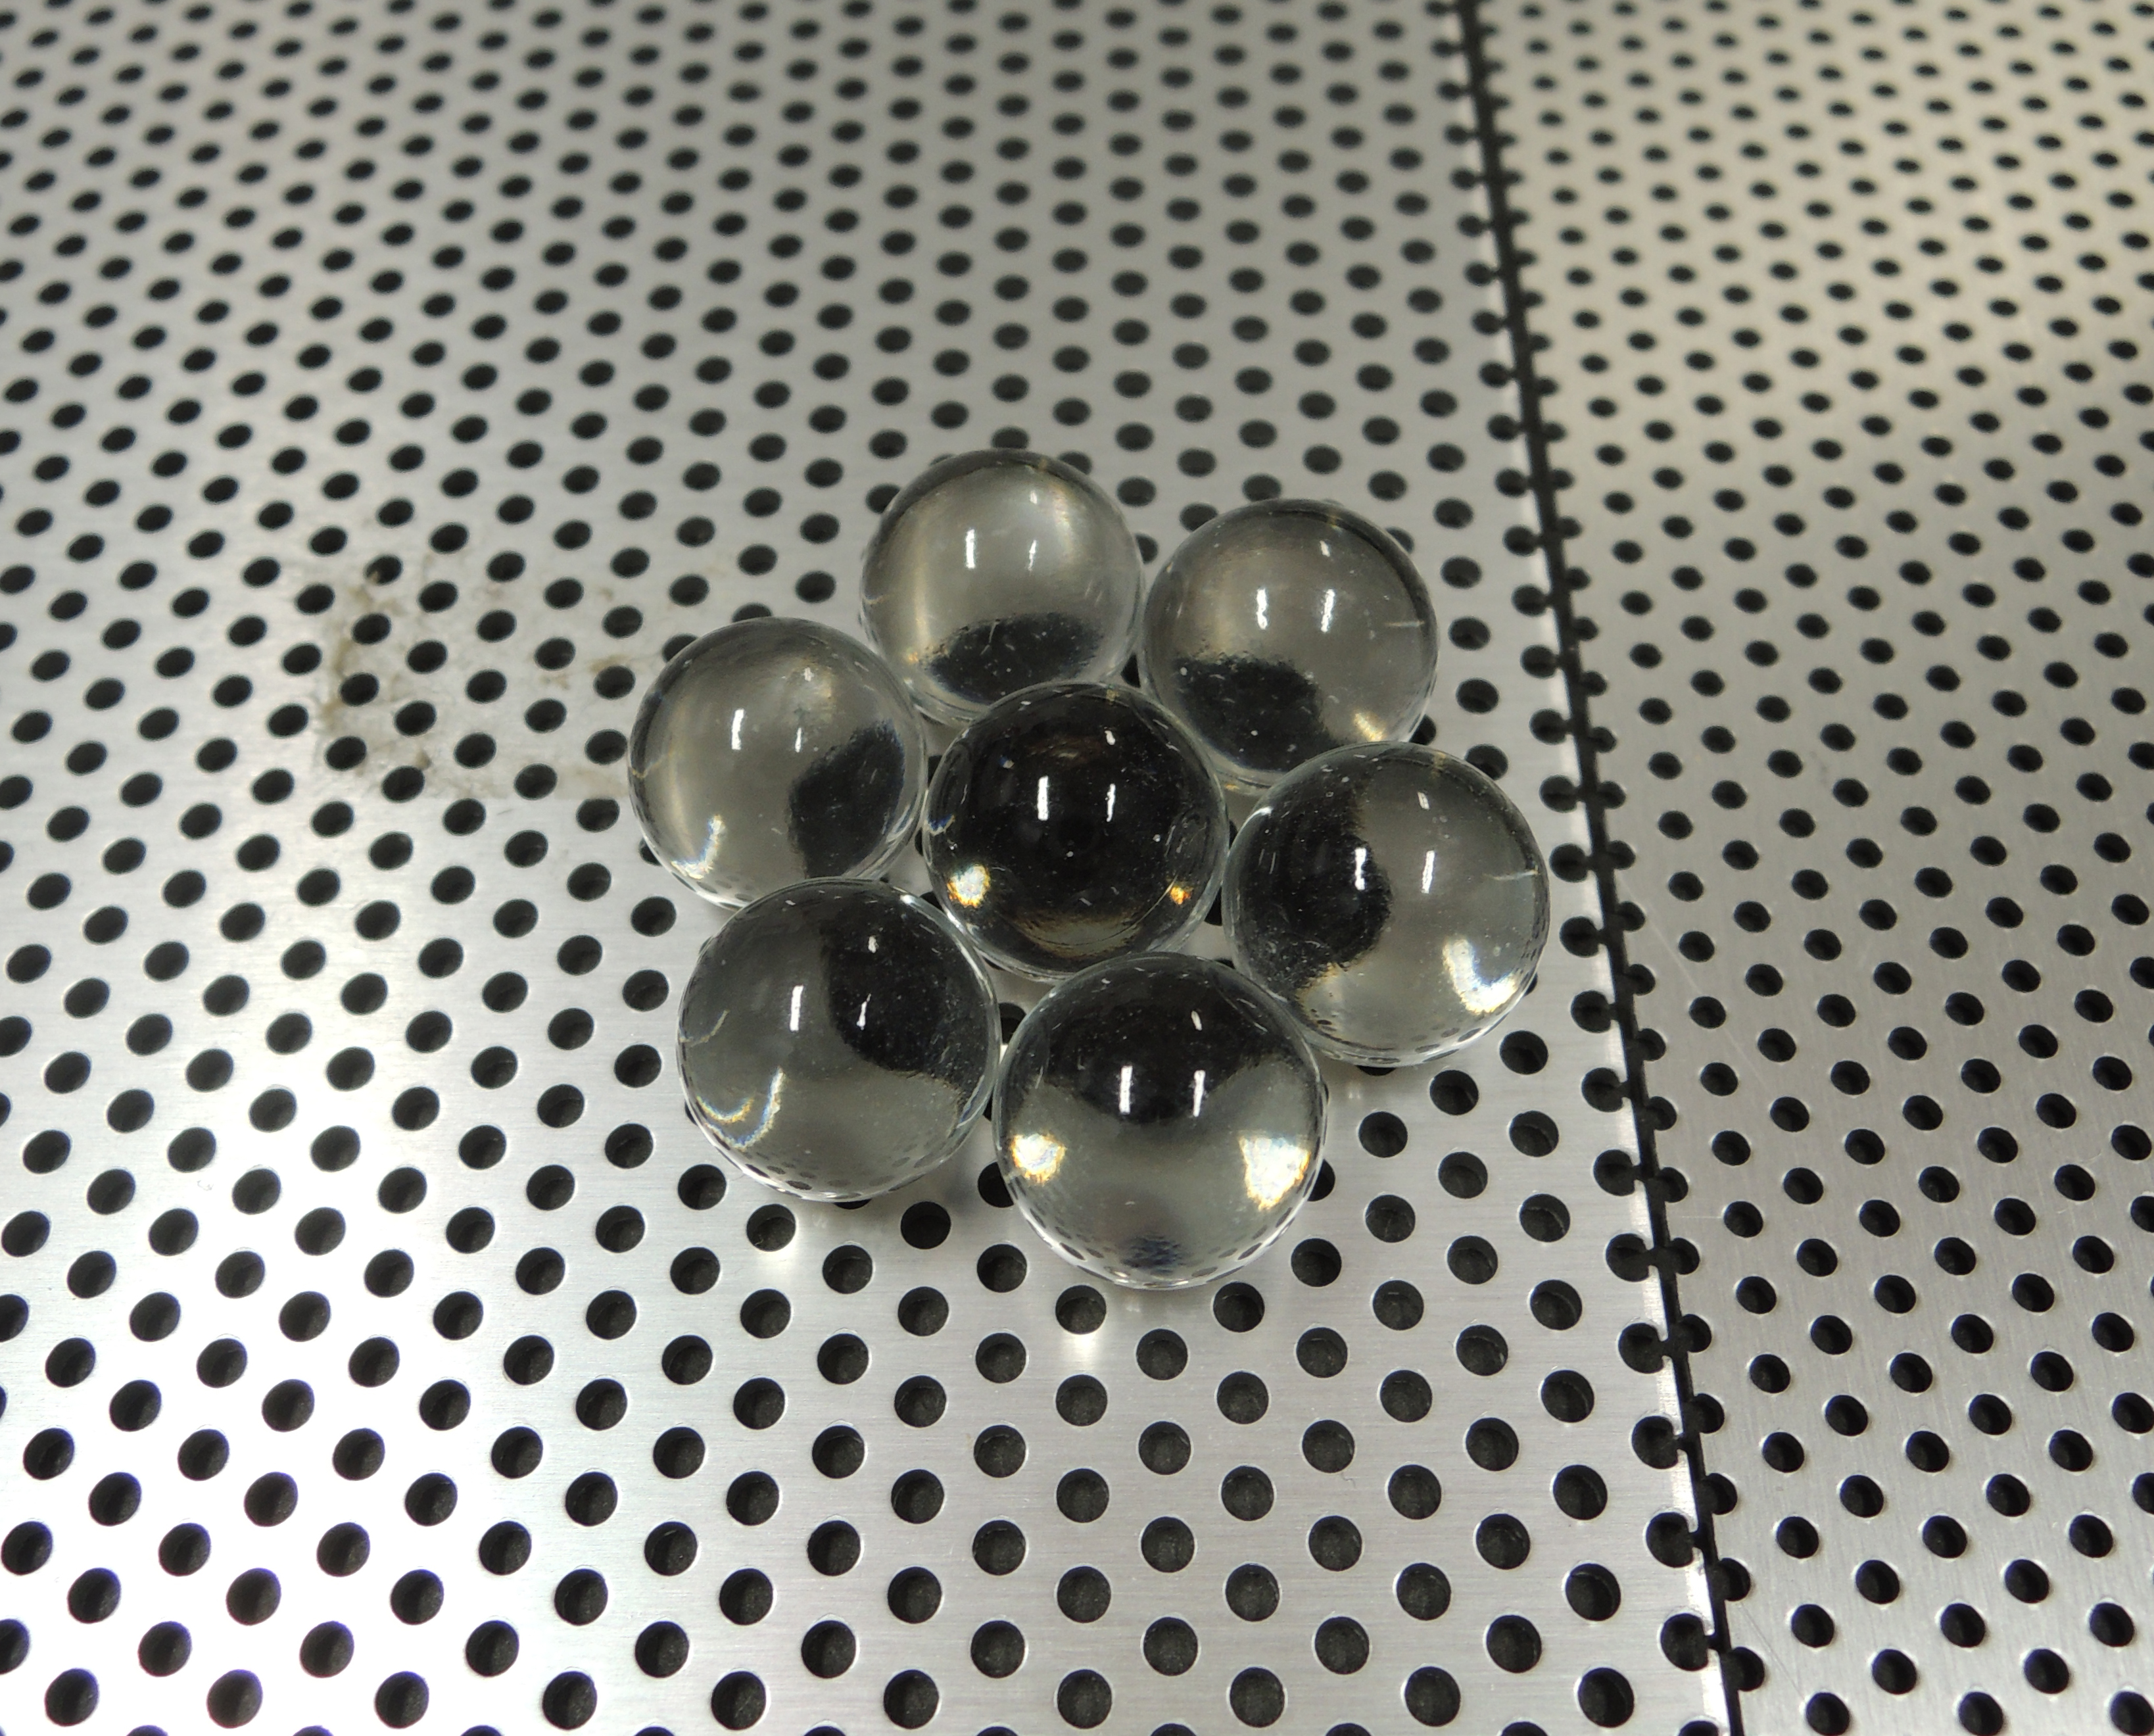
\includegraphics[width=3.5in]{./img/exp_narabe_six.jpg}
%%   \caption{}
%%   \label{FExpNarabeSix}
%% \end{figure}

%% \begin{figure}[htbp]
%%   \centering
%%   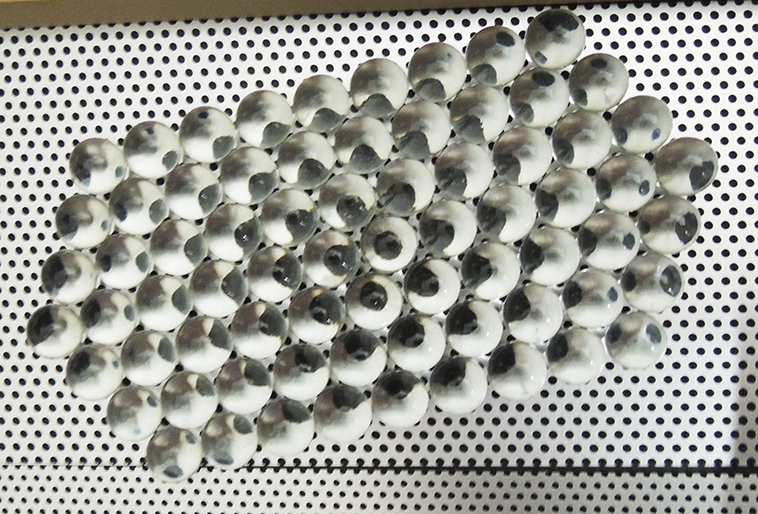
\includegraphics[width=3.5in]{./img/exp_narabe_all.jpg}
%%   \caption{}
%%   \label{FExpNarabeAll}
%% \end{figure}

木枠を用いる方法と比較して、この方法では拡大された黒点をよりはっきりと確認することができる。
その理由として、隣り合う球同士の条件の違いが光源および視点との位置関係のわずかな変化のみであるためだと推測できる。
隣り合う球がお互いに似た像を写すのでノイズが少なく、黒点の拡大像によって全体的に黒くなった複数のビー玉によってひとつのまとまった黒い領域が形成されたり、黒点を写さない複数のビー玉によって広い無色の領域が形成されたりするのであろう\figref{}。

%% \begin{figure}[htbp]
%%   \centering
%% \subfigure[CAPTIONa]{
%% \includegraphics*[width=.45\columnwidth]{./img/exp_res_01.jpg}
%% \label{fig:it-PP}}
%% \subfigure[CAPTIONb]{
%% \includegraphics*[width=.45\columnwidth]{./img/exp_res_02.jpg}
%% \label{fig:st-PP}}\\
%% \subfigure[CAPTIONc]{
%% \includegraphics*[width=.45\columnwidth]{./img/exp_res_03.jpg}
%% \label{fig:at-PP}}
%% \subfigure[CAPTIONd]{
%% \includegraphics*[width=.45\columnwidth]{./img/exp_res_04.jpg}
%% \label{fig:at-PP}}
%%   \caption{}
%%   \label{FExp}
%% \end{figure}

さらに、この方法では視点と実験装置との距離によってひとまとまりの黒点として認識される領域のサイズが大きく変化する。
具体的には、視点が離れるほど黒い領域は大きくなり、視点が近づくほど黒い領域は小さくなる。
%% \begin{figure}[htbp]
%%   \centering
%% \subfigure[CAPTIONa]{
%% \includegraphics*[width=.45\columnwidth]{./img/exp_largespot.png}
%% \label{FExpLargespot}}
%% \subfigure[CAPTIONb]{
%% \includegraphics*[width=.45\columnwidth]{./img/exp_middlespot.png}
%% \label{FExpMiddlespot}}\\
%% \subfigure[CAPTIONc]{
%% \includegraphics*[width=.45\columnwidth]{./img/exp_largespot_circle.png}
%% \label{FExpLargespotCircle}}
%% \subfigure[CAPTIONd]{
%% \includegraphics*[width=.45\columnwidth]{./img/exp_middlespot_circle.png}
%% \label{FExpMiddlespotCircle}}
%%   \caption{CAPTION}
%%   \label{FExp}
%% \end{figure}
\secref{SSOnemarble}の結果から類推すると、ビー玉およびパンチングメタルをある角度前後から観測した場合、ビー玉の表面が黒色で占められると考えられる。
そして、視点が実験装置から離れるほど隣接する球と視線とのなす角度同士の差は小さくなり、視点が近づくほど隣接する球と視点とのなす角度同士の差は大きくなる\figref{}。
すなわち、この実験装置上では視円錐のある角度に収まる領域は黒く見えると考えられる\figref{}。
以上の性質は、実物の複眼上に現れる偽瞳孔現象を適切に説明することができ実際の偽瞳孔の観察結果とも合致するため、本研究において利用できる有力なモデルであると考えられる。

\section{まとめ}
\label{SEcperimentTotal}

複眼の性質を表現するための近似モデルを考えるため、永田の実験をもとにビー玉とパンチングメタルを用いて予備実験を行った。
本実験の目的は3つあり、偽瞳孔のしくみを理解すること、実装前にモデルによる偽瞳孔の再現度を確認すること、そしてパラメータによる偽瞳孔の模様の変化を観察することであった。
ビー玉、パンチングメタル、木の棒および画用紙を用いて実験装置を作成し、いくつかのビー玉の配置パターンについてビー玉に写る像の観察を行った。
\secref{SSOnemarble}では、ビー玉の直下および周辺の黒点に対してビー玉が拡大レンズとして作用していることを確認した。
\secref{SSWoodframe}では、密集した球体レンズが奥で接している面を拡大できることを確認した。
\secref{SSMarbleOnHole}では、レンズと黒点の位置を合わせることで拡大された黒点がよりはっきりと写ることと、その黒い領域が視点と実験装置との距離によって大きさを変えることを確認した。

偽瞳孔が生じるしくみは、個眼の凸レンズの拡大効果によって色素細胞の虚像が見えることによるものであると考えられる。
レンズが密集して並ぶことでそれぞれの個眼が集合し、大きな偽瞳孔の黒点として現れる。
個眼のレンズを球体であるビー玉で代替し、色素細胞を平面であるパンチングメタルに置き換えたモデルにおいても、偽瞳孔と同様の現象を確認した。
個眼に相当するビー玉の大きさよりもおおきくはっきりとした黒色の領域を黒点の像として観測し、再現性としても実際の偽瞳孔と比較しても遜色のない結果を得ることができたと考えられる。
球の大きさや黒点の配置などによる違いを確認することもでき、並んだ黒点同士の距離や表面と視点との距離が巨視的な偽瞳孔の模様に影響を与えることがわかった。
本研究では、\secref{SSMarbleOnHole}の場合を参考に複眼のモデル化を行い、アルゴリズムを考案する。
